
% v2-acmsmall-sample.tex, dated March 6 2012
% This is a sample file for ACM small trim journals
%
% Compilation using 'acmsmall.cls' - version 1.3 (March 2012), Aptara Inc.
% (c) 2010 Association for Computing Machinery (ACM)
%
% Questions/Suggestions/Feedback should be addressed to => "acmtexsupport@aptaracorp.com".
% Users can also go through the FAQs available on the journal's submission webpage.
%
% Steps to compile: latex, bibtex, latex latex
%
% For tracking purposes => this is v1.3 - March 2012
\documentclass[prodmode,acmtecs]{acmsmall} % Aptara syntax
\usepackage[spanish,polish]{babel}
\usepackage[T1]{fontenc}
\usepackage{fancyvrb}
\usepackage{graphicx,hyperref}
\newcommand\cutout[1]{}


\usepackage[table]{xcolor}
\usepackage[utf8]{inputenc}
\usepackage[parfill]{parskip}
\usepackage{tabulary}
\PassOptionsToPackage{hyphens}{url}
\usepackage{hyperref}    
\usepackage[capitalize]{cleveref}


% Metadata Information
% !!! TODO: SET THESE VALUES !!!
\acmVolume{0}
\acmNumber{0}
\acmArticle{CFP}
\acmYear{0}
\acmMonth{0}

\newcounter{colstart}
\setcounter{page}{4}

\RecustomVerbatimCommand{\VerbatimInput}{VerbatimInput}%
{
%fontsize=\footnotesize,
fontfamily=\rmdefault
}


\newcommand{\UnderscoreCommands}{%\do\verbatiminput%
\do\citeNP \do\citeA \do\citeANP \do\citeN \do\shortcite%
\do\shortciteNP \do\shortciteA \do\shortciteANP \do\shortciteN%
\do\citeyear \do\citeyearNP%
}

\usepackage[strings]{underscore}



% Document starts
\begin{document}


\setcounter{colstart}{\thepage}

\acmArticle{CFP}
\title{{\huge\sc SIGLOG Monthly 236}

 April 2023}
\author{DAVID PURSER\affil{University of Liverpool, UK}
\vspace*{-2.6cm}\begin{flushright}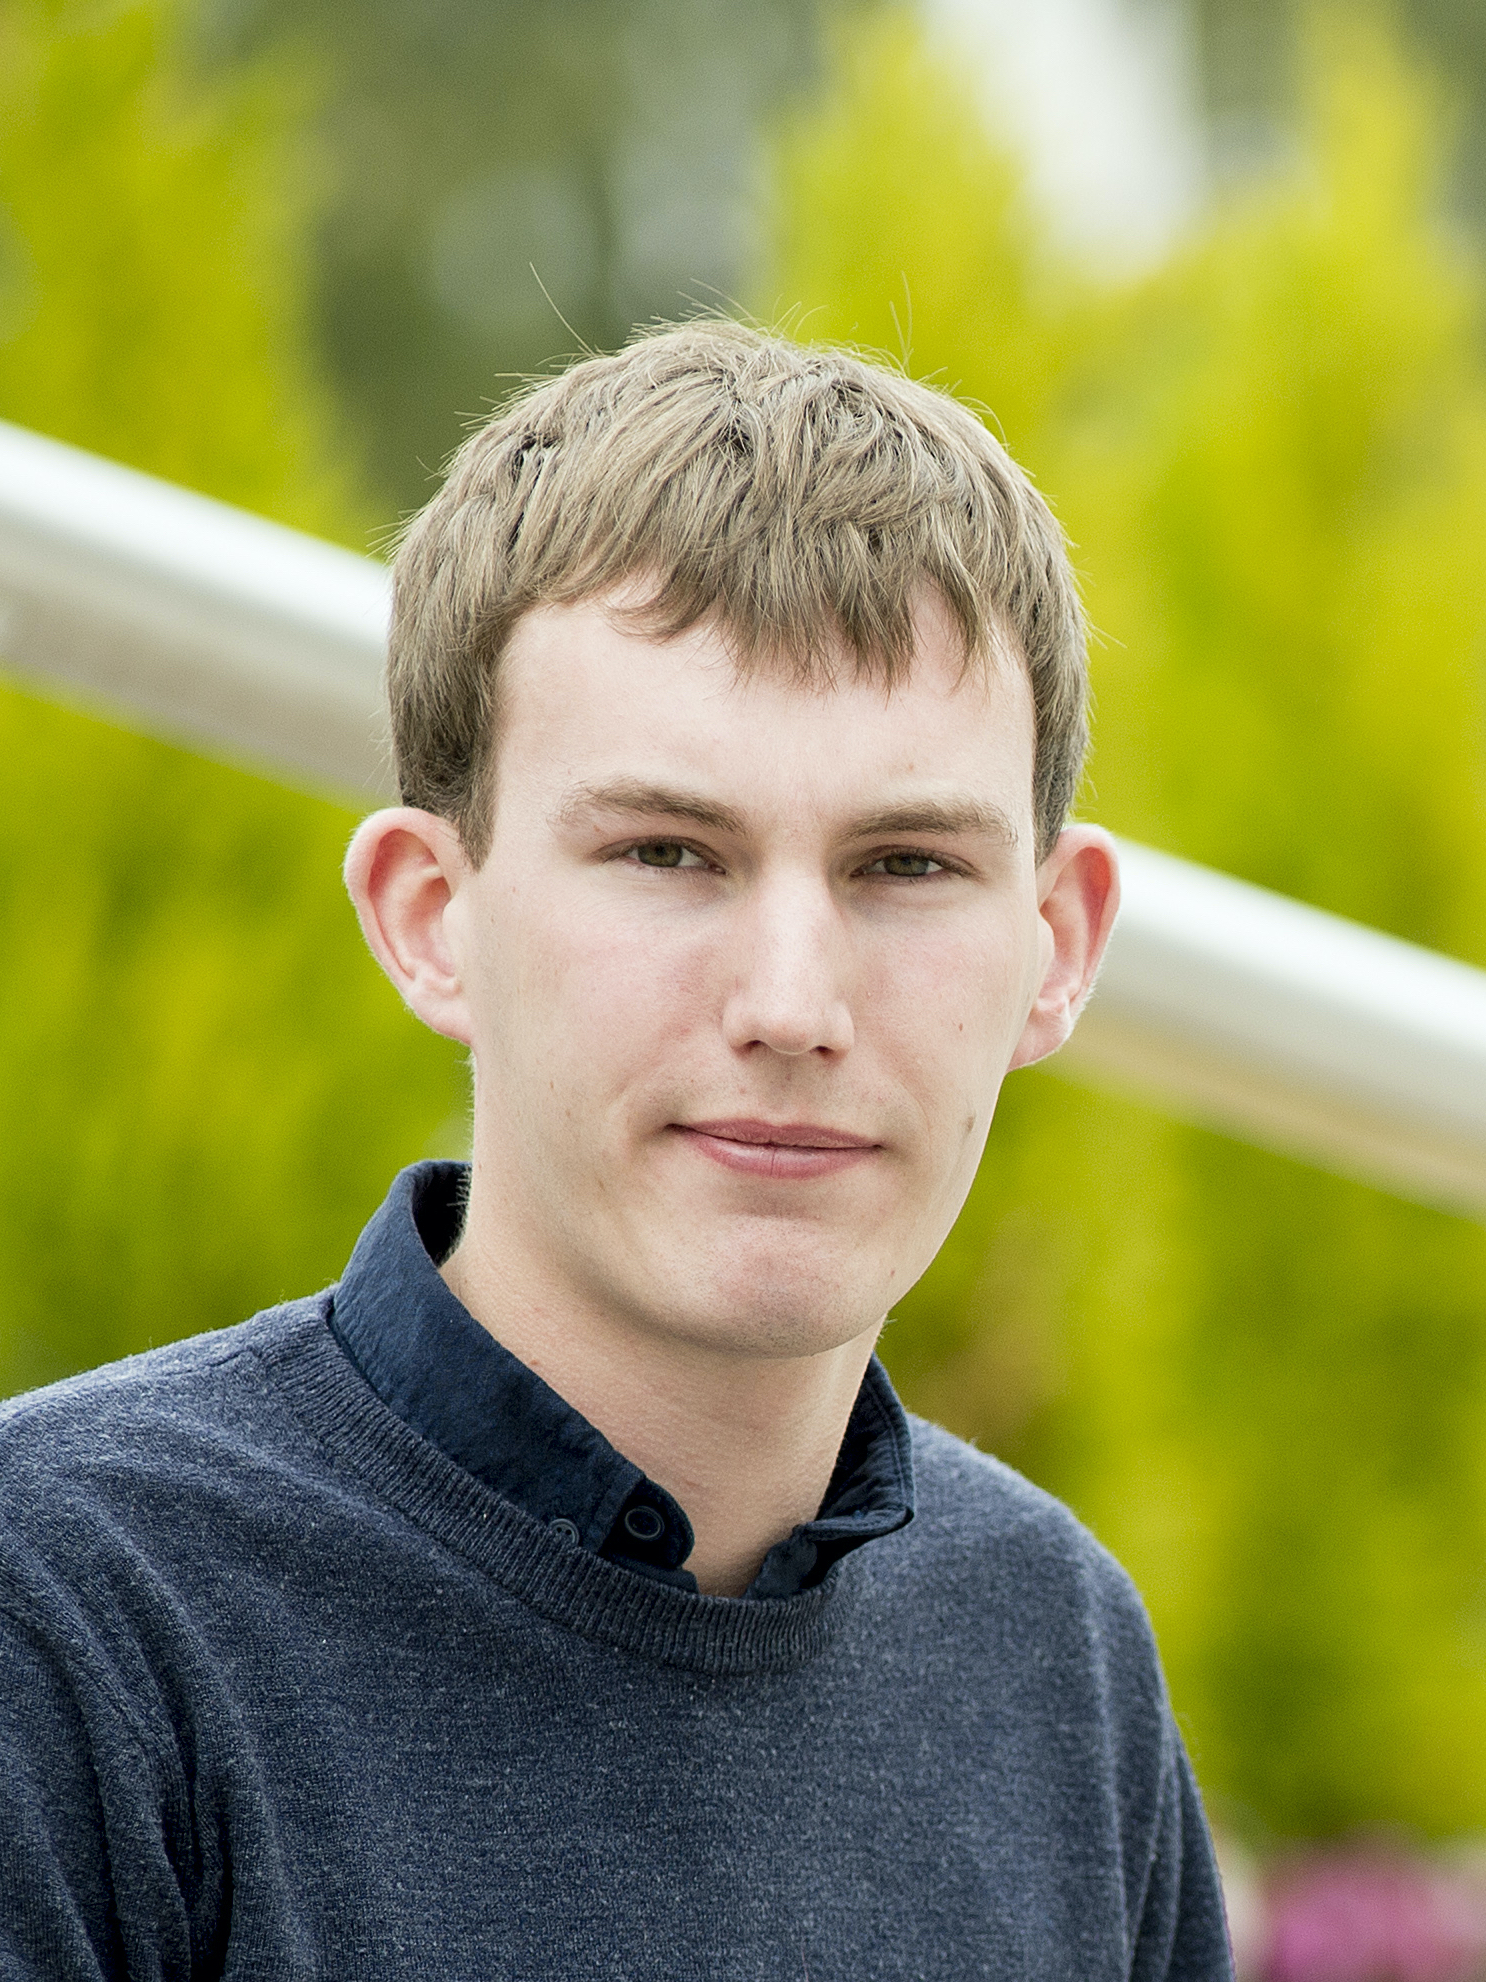
\includegraphics[width=30mm]{dp}\end{flushright}
}

\begin{abstract}
April 2023 edition of SIGLOG Monthly, featuring deadlines, calls and community announcements.
\end{abstract}


\maketitlee

\href{https://lics.siglog.org/newsletters/}{Past Issues}
 - 
\href{https://lics.siglog.org/newsletters/inst.html}{How to submit an announcement}
\section{Table of Content}\begin{itemize}\item DEADLINES (\cref{deadlines}) 
 
\item CALLS 
 
\begin{itemize}\item TAYSIR (CALL FOR PARTICIPATION) (\cref{TAYSIR})
\item UNIF 2023 (CALL FOR PAPERS) (\cref{UNIF2023})
\item WPTE 2023 (CALL FOR PAPERS) (\cref{WPTE2023})
\item MFCS 2023 (CALL FOR PAPERS) (\cref{MFCS2023})
\item CONCUR 2023 (CALL FOR PAPERS) (\cref{CONCUR2023})
\item HIGHLIGHTS’23 (CALL FOR PRESENTATIONS) (\cref{HIGHLIGHTS23})
\item TIME 2023 (CALL FOR PAPERS) (\cref{TIME2023})
\item Twelfth Summer School on Formal Techniques and First Formal Methods in the Field Bootcamp (CALL FOR PARTICIPATION) (\cref{TwelfthSummerSchoolonFormalTechniquesandFirstFormalMethodsintheFieldBootcamp})
\item LICS 2023 Workshop on Combinatorial Games in Finite Model Theory (CALL FOR CONTRIBUTIONS AND PARTICIPATION) (\cref{LICS2023WorkshoponCombinatorialGamesinFiniteModelTheory})
\item EUMAS 2023 (CALL FOR PAPERS) (\cref{EUMAS2023})
\item iFM 2023 (CALL FOR PAPERS) (\cref{iFM2023})
\item ESSLLI (CALL FOR PARTICIPATION) (\cref{ESSLLI})
\item GandALF 23 (CALL FOR PAPERS) (\cref{GandALF23})
\item ACKERMANN AWARD 2023 (CALL FOR NOMINATIONS) (\cref{ACKERMANNAWARD2023})
\item The Proof Society Summer School and affiliated Workshop (CALL TO SAVE THE DATE) (\cref{TheProofSocietySummerSchoolandaffiliatedWorkshop})
\end{itemize} 
\item JOB ANNOUNCEMENTS 
 
\begin{itemize}\item Postdoc at Penn State (\cref{PostdocatPennState})
\item Postdoc on challenging problems in infinite-state systems (\cref{Postdoconchallengingproblemsininfinitestatesystems})
\item PhD or Postdoc Position at LMU Munich about Verified Modal Logics (\cref{PhDorPostdocPositionatLMUMunichaboutVerifiedModalLogics})
\item Two open positions of logic at Zhejiang University in 2023. (\cref{TwoopenpositionsoflogicatZhejiangUniversityin2023})
\end{itemize} 
\end{itemize}\section{Deadlines}\label{deadlines}\rowcolors{1}{white}{gray!25}\begin{tabulary}{\linewidth}{LL}Postdoc at Penn State:  & Mar 31, 2023 (Deadline (not strict)) \\
CLAR 2023:  & Apr 10, 2023 (Submission deadline) \\
VCLA International Student Awards:  & Apr 11, 2023 (Submission deadline, EXTENDED) \\
InqBnB4 workshop:  & Apr 14, 2023 (Submission deadline) \\
Postdoc on challenging problems in infinite-state systems:  & Apr 14, 2023 (Deadline) \\
MARKTOBERDORF 2023:  & Apr 15, 2023 (Registration deadline) \\
PhD or Postdoc Position at LMU Munich about Verified Modal Logics:  & Apr 15, 2023 (Application deadline) \\
FORMATS 2023:  & Apr 21, 2023 (Abstract), Apr 28, 2023 (Paper) \\
UNIF 2023:  & Apr 21, 2023 (Paper Submission) \\
WPTE 2023:  & Apr 21, 2023 (Paper) \\
WiL 2023:  & Apr 23, 2023 (Abstract) \\
MFCS 2023:  & Apr 24, 2023 (Abstract), Apr 28, 2023 (Paper) \\
CONCUR 2023:  & Apr 24, 2023 (Abstract), May 02, 2023 (Paper) \\
HIGHLIGHTS’23:  & Apr 25, 2023 (Regular) \\
ICLP 2023:  & Apr 28, 2023 (non-regular paper) \\
RSSRail 2023:  & Apr 28, 2023 (Abstract for all papers), Apr 28, 2023 (Abstract for tutorials), May 05, 2023 (Full paper) \\
TIME 2023:  & Apr 28, 2023 (Abstract), May 05, 2023 (Paper) \\
TAYSIR:  & Apr 30, 2023 (End of competition) \\
Twelfth Summer School on Formal Techniques and First Formal Methods in the Field Bootcamp:  & Apr 30, 2023 (Recommended Application deadline) \\
LICS 2023 Workshop on Combinatorial Games in Finite Model Theory:  & May 01, 2023 (Abstract Submission) \\
HOR 2023:  & May 02, 2023 (Submission deadline) \\
ACT 2023:  & May 03, 2023 (Submission Deadline) \\
GCM 2023:  & May 07, 2023 (Abstract), May 14, 2023 (Paper) \\
LORI 2023:  & May 15, 2023 (Paper deadline) \\
EUMAS 2023:  & May 20, 2023 (Papers) \\
iFM 2023:  & May 25, 2023 (Abstract) \\
FSCD 2025:  & May 27, 2023 (Deadline for location proposals) \\
ESSLLI:  & May 31, 2023 (Early-registration deadline) \\
Two open positions of logic at Zhejiang University in 2023.:  & May 31, 2023 (Application deadline) \\
GandALF 23:  & Jun 23, 2023 (Abstract), Jun 30, 2023 (Paper) \\
ACKERMANN AWARD 2023:  & Jul 01, 2023 (Deadline for) \\
ICDT 2024:  & Sep 13, 2023 (Cycle 2 Abstract), Sep 20, 2023 (Cycle 2 Full) \\
\end{tabulary}
\section{TAYSIR: Transformer+RNN Algorithms to Yield Simple and Interpretable Representation}\label{TAYSIR}  Competition has started and will last until April 30th 2023. \\ 
  \href{https://remieyraud.github.io/TAYSIR/}{https://remieyraud.github.io/TAYSIR/} \\ 
CALL FOR PARTICIPATION 

\begin{itemize}\item  The Transformers+RNN: Algorithms to Yield Simple and Interpretable Representations (TAYSIR) competition is an on-line challenge on extracting simpler models from already trained neural networks. These neural nets are trained on tasks involving sequences of symbols. Some of these tasks are artificial and some come from real world problems in domains like natural language processing (NLP), bioinformatics, software engineering and others. Taysir means ``simple'' in Arabic. 
 
  The quality of the extracted models is evaluated in two ways: 
 
\begin{itemize}\item  How well the extracted model approximates the original model
\item  The simplicity of the extracted model as measured by assorted metrics
\end{itemize} 
  There are two tracks in the competition corresponding to the kind of function the trained neural networks produce.  
 
\begin{itemize}\item  Neural nets trained for binary classification. These networks represent functions Σ* ➝ \{0,1\}. This task can be thought of as extracting models for formal languages.
\item  Neural nets trained for language modeling and used as density estimators. These networks represent functions Σ* ➝ ℝ. 
\end{itemize} 
  Each track consists of about 10 trained models. The trained models are in PyTorch but available in a MLFlow format for compatibility with other frameworks. 
 
  The competition has started and will last until April 30th 2023. 
 
  Half a day will be dedicated to the competition results during the 16th International Conference on Grammatical Inference to be held in Morocco in July 2023 at the Faculty of Sciences, Mohammed V University in Rabat, Morocco. 
 
  \href{http://www.fsr.ac.ma/icgi2023/}{http://www.fsr.ac.ma/icgi2023/} 
 
  Participants in TAYSIR will be encouraged to attend ICGI 2023 and to submit an extended abstract presenting their work (2 to 4 pages, including appendices) by May 15th which will be appended to the proceedings of ICGI (publisher: PMLR) in a track dedicated to the competition. These abstracts will be peer-reviewed primarily for clarity of presentation. 
 
\item  HOW TO PARTICIPATE 
 
  Everything can be found on our website: \href{https://remieyraud.github.io/TAYSIR/}{https://remieyraud.github.io/TAYSIR/}  
 
\end{itemize}\section{UNIF 2023: 37th INTERNATIONAL WORKSHOP ON UNIFICATION}\label{UNIF2023}  July 2, 2023, Rome, Italy\\ 
  A satellite workshop of CADE/FSCD, affiliated with FSCD\\ 
  \href{https://project.inria.fr/unif2023}{https://project.inria.fr/unif2023}\\ 
CALL FOR PAPERS 

\begin{itemize}\item  The International Workshop on Unification (UNIF) is a yearly forum 
 
  devoted to unification theory and its applications. Unification is 
 
  concerned with the problem of identifying terms, finding solutions 
 
  for equations, or making formulas equivalent. It is a fundamental 
 
  process used in a number of fields of computer science, including 
 
  automated reasoning, term rewriting, logic programming, natural 
 
  language processing, program analysis, types, etc. 
 
\item  A non-exhaustive list of topics of interest includes: syntactic and 
 
  equational unification; matching; constraint solving; unification in 
 
  modal, temporal, and description logics; narrowing; disunification; 
 
  anti-unification; semi-unification; higher-order unification; 
 
  complexity issues; implementation techniques; applications. 
 
\item  IMPORTANT DATES: 
 
\rowcolors{1}{white}{gray!25}\begin{tabulary}{\linewidth}{LL}Paper Submission:  & Apr 21, 2023 \\
Author notification:  & May 26, 2023 \\
Final version:  & Jun 09, 2023 \\
\end{tabulary}
 
\item  INVITED SPEAKERS:  
 
\begin{itemize}\item  Mauricio Ayala-Rincon (Universidade de Brasilia)
\item  Deepak Kapur (UNM, Albuquerque)
\end{itemize} 
\item  Detailed information can be found on the webpage 
 
\end{itemize}\section{WPTE 2023: 10th International Workshop on Rewriting Techniques for Program Transformations and Evaluation}\label{WPTE2023}  July 1, 2023, Rome, Italy\\ 
  \href{https://wpte2023.github.io/}{https://wpte2023.github.io/}\\ 
  \href{https://easychair.org/conferences/?conf=wpte2023}{https://easychair.org/conferences/?conf=wpte2023}\\ 
CALL FOR PAPERS 

\begin{itemize}\item  The aim of WPTE is to bring together the researchers working on program transformations, evaluation, and operationally based programming language semantics, using rewriting methods, in order to share the techniques and recent developments and to exchange ideas to encourage further activation of research in this area. 
 
\item  Topics include: correctness of program transformations, optimizations and translations; program transformations for proving termination, confluence, and other properties; correctness of evaluation strategies; operational semantics of programs, operationally-based program equivalences such as contextual equivalences and bisimulations; cost-models for arguing about the optimizing power of transformations and the costs of evaluation; program transformations for verification and theorem proving purposes; translation, simulation, equivalence of programs with different formalisms, and evaluation strategies; program transformations for applying rewriting techniques to programs in specific programming languages; program transformations for program inversions and program synthesis; program transformation and evaluation for Haskell and rewriting. 
 
\item  IMPORTANT DATES: (AoE) 
 
\rowcolors{1}{white}{gray!25}\begin{tabulary}{\linewidth}{LL}Paper submission:  & Apr 21, 2023 \\
Notifications:  & May 22, 2023 \\
Final version for informal proceedings:  & Jun 10, 2023 \\
Workshop:  & Jul 01, 2023 \\
Submission to post-proceedings (journal):  & Autumn 2023 (tbc) \\
\end{tabulary}
 
\end{itemize}\section{MFCS 2023: 48th International Symposium on Mathematical Foundations of Computer Science}\label{MFCS2023}  August 28 — September 1, 2023, Bordeaux, France\\ 
  \href{https://mfcs2023.labri.fr}{https://mfcs2023.labri.fr}\\ 
CALL FOR PAPERS 

\begin{itemize}\item  The MFCS conference series on Mathematical Foundations of Computer Science is a high-quality venue for original research in all branches the longest history in the field-the first conference in the series was held already in 1972. Traditionally, the conference moved between the Czech Republic, Slovakia, and Poland, while since 2013, the conference has traveled around Europe. MFCS 2023 will be held in Bordeaux, France. 
 
  Barring substantial and unforeseen developments, MFCS will be organized as a physical event, and at least one author of each accepted paper must register at the conference. 
 
\item  IMPORTANT DATES (AOE) 
 
\rowcolors{1}{white}{gray!25}\begin{tabulary}{\linewidth}{LL}Abstract submission:  & Apr 24, 2023 \\
Paper submission:  & Apr 28, 2023 \\
Notification of authors:  & Jun 27, 2023 \\
Camera-ready:  & Jul 18, 2023 \\
Conference dates:  & Aug 28-Sep 1, 2023 \\
\end{tabulary}
 
\item  SUBMISSION GUIDELINES 
 
  Papers should be submitted electronically through EasyChair. \href{https://easychair.org/my/conference?conf=mfcs2023}{https://easychair.org/my/conference?conf=mfcs2023} 
 
  LIPIcs Style mandatory, max 12 pages (excluding references and appendix to be consulted at the discretion of the program committee). 
 
  No prior publication or simultaneous submission (except preprint repositories such as arXiv or workshops without formal published proceedings). 
 
\item  LIST OF TOPICS 
 
  We encourage submission of original research papers in all areas of theoretical computer science, including (but not limited to) the following: algebraic and co-algebraic methods in computer science; algorithms and data structures; automata and formal languages; bioinformatics; combinatorics on words, trees, and other structures; computational complexity (structural and model-related); computational geometry; computer-aided verification; computer assisted reasoning; concurrency theory; cryptography and security; cyber physical systems, databases and knowledge-based systems; formal specifications and program development; foundations of computing; logics in computer science; mobile computing; models of computation; networks; parallel and distributed computing; quantum computing; semantics and verification of programs; theoretical issues in artificial intelligence and machine learning; types in computer science 
 
\end{itemize}\section{CONCUR 2023: the 34th International Conference on Concurrency Theory}\label{CONCUR2023}  September 19-22, 2023, University of Antwerp, Belgium\\ 
  Part of CONFEST 2023\\ 
  \href{https://www.uantwerpen.be/en/conferences/confest-2023/concur/}{https://www.uantwerpen.be/en/conferences/confest-2023/concur/}\\ 
CALL FOR PAPERS 

\begin{itemize}\item  CONCUR 2023 solicits high quality papers reporting research results and/or experience related to the topics mentioned below. All papers must be original, unpublished, and not submitted for publication elsewhere. 
 
\item  SUBMISSION  
 
  Full submission information can be found at \href{https://www.uantwerpen.be/en/conferences/confest-2023/concur/call/}{https://www.uantwerpen.be/en/conferences/confest-2023/concur/call/} 
 
\item  IMPORTANT dates (anywhere on Earth) 
 
\rowcolors{1}{white}{gray!25}\begin{tabulary}{\linewidth}{LL}Abstract submission:  & Apr 24, 2023 \\
Paper submission:  & May 02, 2023 \\
Rebuttal Response:  & Jun 5-9, 2023 \\
Notification:  & Jun 28, 2023 \\
Camera Ready:  & Jul 12, 2023 \\
Conference(s):  & Sep 17-22, 2023 \\
Workshops:  & Sep 18+23, 2023 \\
\end{tabulary}
 
\item  TOPICS 
 
  Submissions are solicited in semantics, logics, verification and analysis of concurrent systems. The principal topics include (but are not limited to): 
 
\begin{itemize}\item  Basic models of concurrency such as abstract machines, domain-theoretic models, game-theoretic models, process algebras, graph transformation systems, Petri nets, hybrid systems, mobile and collaborative systems, probabilistic systems, real-time systems, biology-inspired systems, and synchronous systems;
\item  Logics for concurrency such as modal logics, probabilistic and stochastic logics, temporal logics, and resource logics;
\item  Verification and analysis techniques for concurrent systems such as abstract interpretation, atomicity checking, model checking, race detection, pre-order and equivalence checking, run-time verification, state-space exploration, static analysis, synthesis, testing, theorem proving, type systems, and security analysis; 
\item  Distributed algorithms and data structures: design, analysis, complexity, correctness, fault tolerance, reliability, availability, consistency, self-organization, self-stabilization, protocols;
\item  Theoretical foundations of architectures, execution environments, and software development for concurrent systems such as geo-replicated systems, communication networks, multiprocessor and multi-core architectures, shared and transactional memory, resource management and awareness, compilers and tools for concurrent programming, programming models such as component-based, object- and service-oriented.
\end{itemize} 
\end{itemize}\section{HIGHLIGHTS’23: HIGHLIGHTS OF LOGIC, GAMES, AND AUTOMATA}\label{HIGHLIGHTS23}  Kassel, Germany, 24 — 28 July 2023\\ 
  \href{https://highlights-conference.org/2023/}{https://highlights-conference.org/2023/}\\ 
CALL FOR PRESENTATIONS 

\begin{itemize}\item  HIGHLIGHTS’23 is the eleventh in the series of international conferences “Highlights of Logic, Games and Automata”, aiming at integrating the community working in algorithmic model theory, automata theory, databases, games for logic and verification, logic, and verification. Papers from these areas are dispersed across many conferences, which makes them difficult to follow. A visit to the HIGHLIGHTS conference should offer a wide picture of the latest research in the field and a chance to meet everybody in the community, not just those who happen to publish in one particular proceedings volume. There are no publications. 
 
  HIGHLIGHTS’23 is scheduled from July 24 to July 28, 2023 at the Campus Center of the University of Kassel, Germany. The main conference will be preceded by the Highlights Collaborative Research Week (HCRW), from July 17 to July 21, 2023 at the Faculty of Electrical Engineering and Computer Science of the University of Kassel. 
 
\item  HIGHLIGHTS’23 key features:  
 
  new: A group chat has been set up to facilitate exchanges among the HIGHLIGHTS community. HIGHLIGHTS is a conference without publication, where speakers give short presentations of their best work.  
 
  new: The conference will span five days, including tutorials.  
 
  new: The Highlights’ Collaborative Research Week (HCRW) is a new initiative meant to facilitate research collaborations/discussions between participants. HCRW is scheduled from July 17 to July 21, 2023, i.e. the week before HIGHLIGHTS’23 and after ICALP’23 (in Paderborn, Germany).  
 
  The Highlights Extended Stay Support Scheme (HESSS) is intended to help participants find collaborators and organize visits around HIGHLIGHTS.  
 
  We encourage you to attend and present your best work, be it already published or not, at HIGHLIGHTS’23. 
 
\item  SCOPE 
 
  Representative areas include, but are not restricted to: Algorithmic model theory Automata theory, Databases, Games for logic and verification, Logic, Verification 
 
\item  IMPORTANT DATES AND INFORMATION 
 
\rowcolors{1}{white}{gray!25}\begin{tabulary}{\linewidth}{LL}Regular submission:  & Apr 25, 2023 \\
Regular notification:  & May 05, 2023 \\
Early registration:  & TBA \\
Highlights’ Collaborative Research Weak (HCRW):  & Jul 17-21, 2023 \\
Conference:  & Jul 24-28, 2023 \\
Tutorial day:  & Jul 24, 2023 \\
\end{tabulary}
 
\item  Before coming from far away, please review how your trip and international flights are contributing to climate change. We encourage you to take the train as much as possible, possibly taking the opportunity for visiting colleagues on the way and thus decomposing the travel into smaller pieces. More generally, we encourage you to make the most of your stay. This means extending your journey to the previous and/or following weeks for more scientific activities in Kassel and around. 
 
\item  SUBMISSIONS AND GUIDELINES 
 
  See the full call for further information: \href{https://highlights-conference.org/2023/}{https://highlights-conference.org/2023/} 
 
\item  TUTORIALS: 
 
\begin{itemize}\item  Bernd Finkbeiner (Saarland Univ and CISPA, Germany) 
\item  Édouard Bonnet (ENS Lyon, France) 
\end{itemize} 
\item  INVITED TALKS: 
 
\begin{itemize}\item  Udi Boker (Reichman Univ, Israel) 
\item  Véronique Bruyère (Univ of Mons, Belgium) 
\item  Meena Mahajan (Institute of Mathematical Sciences, India) 
\item  Sophie Pinchinat (IRISA, France) 
\item  Sven Schewe (Univ of Liverpool, UK)
\end{itemize} 
\end{itemize}\section{TIME 2023: 30th International Symposium on Temporal Representation and Reasoning}\label{TIME2023}  25-26 September, 2023\\ 
  NCSR Demokritos, Athens, Greece\\ 
  \href{https://cer.iit.demokritos.gr/events/time23/}{https://cer.iit.demokritos.gr/events/time23/}\\ 
CALL FOR PAPERS 

\begin{itemize}\item  TIME brings together researchers from different disciplines of Computer Science working on temporal aspects of computational systems. We are happy to announce that TIME is back to an in-person conference! In addition to theoretical work, we invite submissions focusing on the development, deployment and evaluation ofsystems for temporal reasoning. Such systems papers will be evaluated primarily on the quality of the empirical evaluation and reusability. 
 
\item  TOPICS for TIME 2023 include, but are not limited to:  
 
  time in artificial intelligence; time in data science; temporal logic and reasoning; spatial and temporal reasoning; time in natural language processing; reasoning about action and change; complex event recognition and forecasting; planning and planning languages; ontologies of time and space-time; belief and uncertainty in temporal knowledge; temporal learning and discovery; temporal data models and query languages; temporal query processing and indexing; temporal data mining; time-series data management; stream data management; spatio-temporal data management, including moving objects; data currency and expiration; indeterminate and imprecise temporal data; temporal constraints; specification and verification of systems; verification of software and web applications; synthesis and execution; model checking algorithms and implementations; temporal logics for infinite-state systems; runtime verification of temporal properties; temporal aspects of agent- and policy-based systems; temporal networks. 
 
\item  IMPORTANT DATES: 
 
\rowcolors{1}{white}{gray!25}\begin{tabulary}{\linewidth}{LL}Abstract submission:  & Apr 28, 2023 \\
Paper submission:  & May 05, 2023 \\
Notification:  & Jun 16, 2023 \\
\end{tabulary}
 
\item  SUBMISSION: 
 
  See submission information at \href{https://cer.iit.demokritos.gr/events/time23/#submissions}{https://cer.iit.demokritos.gr/events/time23/\#submissions} 
 
\end{itemize}\section{Twelfth Summer School on Formal Techniques and First Formal Methods in the Field Bootcamp}\label{TwelfthSummerSchoolonFormalTechniquesandFirstFormalMethodsintheFieldBootcamp}  Twelfth Summer School on Formal Techniques: May 24 - May 28, 2023 (\href{http://fm.csl.sri.com/SSFT23}{http://fm.csl.sri.com/SSFT23}) \\ 
  First Formal Methods in the Field Bootcamp: May 29-June 2, 2023\\ 
CALL FOR PARTICIPATION 

\begin{itemize}\item  Techniques based on formal logic, such as model checking, satisfiability, static analysis, and automated theorem proving, are finding a broad range of applications in modeling, analysis, verification, and synthesis. This school, the twelfth in the series, will focus on the principles and practice of formal techniques, with a strong emphasis on the hands-on use and development of this technology. It primarily targets graduate students and young researchers who are interested in studying and using formal techniques in their research.  A prior background in formal methods is helpful but not required. Participants at the school can expect to have a seriously fun time experimenting with the tools and techniques presented in the lectures during laboratory sessions.  
 
  This year, 2023, we celebrate the 60th anniversary of Alan Robinson's first publication on Resolution, and are delighted to have a series of lectures devoted to the latest developments in this important strand of automated reasoning.  The summer school will be immediately followed by a Formal Methods in the Field (FMiTF) Bootcamp.  Participants in the Bootcamp will employ formal tools and techniques (including those taught in this and prior summer school editions) under the supervision of the Bootcamp faculty to create verified artifacts. 
 
\item  LECTURERS  
 
\begin{itemize}\item  Pamela Zave (Princeton) and Tim Nelson (Brown): No More Garbage In:  Validating Formal Models 
\item  Laura Kovacs (TU Wien) and Andrei Voronkov (Manchester): First-Order Theorem Proving 
\item  Geoff Sutcliffe (Miami): The TPTP World - Infrastructure for Automated Reasoning 
\item  Natarajan Shankar and Stephane Graham-Lengrand (SRI CSL): Speaking Logic
\end{itemize} 
  In addition, we have distinguished invited talks:  
 
\begin{itemize}\item  Maria Paola Bonacina, Università degli Studi di Verona: Resolution, Unification, and Subsumption: Fundamental Concepts in Theorem Proving 
\item  Leslie Lamport (MSR): Q \& A on Paxos 
\item  Jesse Michael Han (OpenAI):: Language Model Software and the Future of Verified Programming
\end{itemize} 
  The Formal Methods in the Field Bootcamp will be held following the summer school from May 29 to the morning of June 2, 2023.  This edition of the FMiTF Bootcamp will be taught by SRI staff with expertise spanning a range of tools covering static and dynamic analyzers, code verifiers, rewrite engines, SAT/SMT solvers, interactive proof assistants, and model checkers. 
 
\item  This year, the school/bootcamp will take place in a hybrid mode: the lectures and labs will be live-streamed and recorded. We strongly encourage in-person participation so that you can benefit from interactions outside the classroom. We have funding from NSF to cover transportation/food/lodging expenses for selected US-based students. Non-student and non-US in-person participants are expected to cover their own transportation and will be charged a fee (around $150/day) to cover the cost of food and lodging. 
 
  The registration link is at the URL: \href{http://fm.csl.sri.com/SSFT23}{http://fm.csl.sri.com/SSFT23}. Participants can register separately for the school and the bootcamp. 
 
  The 2023 Summer School on Formal Techniques will be presented in a hybrid format.  We encourage those students who can attend in person to do so.  Those who cannot be there in person can still participate virtually but they will need to synchronize with the Pacific Daylight Savings Time. Applications should be submitted together with names of two references (preferably advisors, professors, or senior colleagues). 
 
  Applicants are urged to submit their applications before April 30, 2023, since there are only a limited number of spaces available.  Those needing invitation letters for visa purposes are encouraged to complete their applications as early as possible.  We strongly encourage the participation of women and under-represented minorities in the summer school.  
 
Recommended Application deadline: Apr 30, 2023 
 
\end{itemize}\section{LICS 2023 Workshop on Combinatorial Games in Finite Model Theory}\label{LICS2023WorkshoponCombinatorialGamesinFiniteModelTheory}  June 24-25, 2023, Boston, USA\\ 
  \href{https://gamesandfmt.org/workshop2023/}{https://gamesandfmt.org/workshop2023/}\\ 
CALL FOR CONTRIBUTIONS AND PARTICIPATION 

\begin{itemize}\item  The goal of this workshop is to promote work at the interface of complexity and logic. The workshop has two main foci: the first is recent progress in using combinatorial games to prove logical (in)expressiblity results, the second is limitations in the method of combinatorial games as a tool for establishing lower bounds in computational complexity. 
 
\item  INVITED SPEAKERS 
 
  Yijia Chen (Shanghai Jiao Tong University),  Erich Grädel (RWTH Aachen), Neil Immerman (University of Massachusetts Amherst), Antonina Kolokolova (Memorial University of Newfoundland) 
 
\item  SUBMISSION GUIDELINES 
 
  Those wishing to speak at the workshop on any topic related to combinatorial games in finite model theory are invited to submit an Extended Abstract of up to three pages (including references) describing the content of the contributed presentation. At least one author from each accepted abstract must register for the workshop and present the work in person. For additional information, please visit the workshop webpage \href{https://gamesandfmt.org/workshop2023/}{https://gamesandfmt.org/workshop2023/} 
 
\item  IMPORTANT DATES 
 
\rowcolors{1}{white}{gray!25}\begin{tabulary}{\linewidth}{LL}Abstract Submission:  & May 01, 2023 \\
Author Notification:  & May 15, 2023 \\
Workshop Dates:  & Jun 24, 2023 \\
\end{tabulary}
 
\end{itemize}\section{EUMAS 2023: European Conference on Multi-Agent Systems}\label{EUMAS2023}  University of Naples (September 14-15th, 2023). EUMAS\\ 
  \href{https://vadimmalvone.github.io/eumas2023/}{https://vadimmalvone.github.io/eumas2023/}\\ 
CALL FOR PAPERS 

\begin{itemize}\item  The 20th European Conference on Multi-Agent Systems (EUMAS 2023) will be located at the University of Naples (September 14-15th, 2023). EUMAS 2023 is an EURAMAS designated and aims to encourage and support activity in the research and development of multi-agent systems, in academic and industrial effort. The conference aspires to be the primary European forum for researchers interested in the theory and practice of autonomous agents and multi-agent systems. EUMAS enables researchers to meet, present challenges, preliminary and mature research results in an open environment. EUMAS 2023 features formal proceedings published as part of the Lecture Notes in Computer Science (LNCS) series of Springer 
 
  EUMAS 2023 welcomes original, unpublished papers including improved versions of extended abstracts or rejected papers from AAMAS, AAAI and IJCAI 2023. The submission should describe work that has not been previously published, accepted for publication, nor is currently under review by another conference or journal. 
 
\item  TOPICS of interest include, but are not limited to: 
 
  Action and Planning; Adaptation and Learning; Agent Architectures; Agent Programming Languages; Agent Development Methodologies and Tools; Agent-Based Simulation; Agent Organizations and Institutions; Agent-oriented Software Engineering; Agents and Complex Systems; Applications of Multi-agent Systems; Argumentation; Automated negotiation; Biologically inspired approaches; Cognitive Models; Collective and Swarm Intelligence; Collective Intentionality; Communication, Cooperation, and Coordination - Computational Social Choice; Economic Models; Electronic Commerce; Ethical behavior of multi-agent systems; Formal Modelling; Game-Theoretic Methods - Human-Agent Interaction; Logics for Multi-Agent Systems; Logics for Strategic Reasoning; Negotiation; Self-organization; Semantic Web Agents - Social Networks; Socio-technical Systems; Theories of Agency; Trust and Reputation; Verification; Virtual Agents; Voting and Judgment Aggregation Models for multi-agent systems 
 
\item  SUBMISSIONS 
 
   See full call for details: 
 
   \href{https://vadimmalvone.github.io/eumas2023}{https://vadimmalvone.github.io/eumas2023} 
 
\item  IMPORTANT DATES 
 
\rowcolors{1}{white}{gray!25}\begin{tabulary}{\linewidth}{LL}Papers submission:  & May 20, 2023 \\
Notification:  & Jul 05, 2023 \\
Camera ready papers:  & Jul 20, 2023 \\
\end{tabulary}
 
\end{itemize}\section{iFM 2023: 18th International Conference on integrated Formal Methods}\label{iFM2023}   13-15 November 2023, Leiden, the Netherlands\\ 
   \href{https://ifm23.liacs.nl}{https://ifm23.liacs.nl}\\ 
CALL FOR PAPERS 

\begin{itemize}\item  IMPORTANT DATES 
 
\rowcolors{1}{white}{gray!25}\begin{tabulary}{\linewidth}{LL}Abstract submission:  & May 25, 2023 \\
Paper submission:  & Jun 01, 2023 \\
Acceptance notification:  & Aug 10, 2023 \\
iFM 2023 main conference:  & Nov 13-15, 2023 \\
\end{tabulary}
 
\item  OBJECTIVE AND SCOPE  
 
  In the last decades, we have witnessed a proliferation of approaches that integrate several modelling, verification and simulation techniques, facilitating more versatile and efficient analysis of software-intensive systems. These approaches provide powerful support for the analysis of different functional and non-functional properties of the systems, complex interaction of components of different nature as well as validation of diverse aspects of system behaviour. The iFM conference series is a forum for discussing recent research advances in the development of integrated approaches to formal modelling and analysis. The conference covers all aspects of the design of integrated techniques, including language design, verification and validation, automated tool support and the use of such techniques in software engineering practice. To credit the effort of tool developers, we use EAPLS artefact badging \href{https://eapls.org/pages/artifact_badges/}{https://eapls.org/pages/artifact\_badges/}. 
 
  Areas of interest include (but are not limited to): 
 
\begin{itemize}\item  Formal and semi-formal modelling notations 
\item  Combining formal methods with different performance, simulation and system analysis techniques 
\item  Program verification, model checking, and static analysis 
\item  Theorem proving, decision procedures and SAT/SMT solving 
\item  Runtime analysis, monitoring and testing 
\item  Program synthesis 
\item  Modelling, analysis and synthesis of cyber-physical, hybrid, embedded, probabilistic, distributed or concurrent systems 
\item  Abstraction and refinement 
\item  Model learning and inference 
\item  Approaches to integrating formal methods into software engineering practice or industry 
\item  Approaches to integrating formal methods into standardisation or certification processes 
\item  Formal methods for AI 
\item  Tools and case studies supporting the integration of formal methods 
\end{itemize} 
\item  PAPER CATEGORIES  
 
  iFM 2023 solicits high-quality papers reporting research results and/or experience reports related to the overall theme of formal methods integration. 
 
  We accept papers in the following categories: 
 
\begin{itemize}\item  1) Regular papers (limit 16 pages) on: original scientific research results, tools, their foundation and evaluations, applications of formal methods, including rigorous evaluations
\item  2) Short papers (limit 6 pages) on: any subject of interest in the area of formal methods that can be described with sufficient detail within the page limit
\end{itemize} 
  All page limits exclude the references. Appendices may be included, but they will only be read by a reviewer at their discretion. 
 
  Regular and short papers must be original, unpublished, and not submitted for publication elsewhere. Papers will undergo a thorough review process. Submissions will be judged on the basis of significance, relevance, correctness, originality and clarity. 
 
  See full call for submission information: \href{https://liacs.leidenuniv.nl/~bonsanguemm/ifm23/calls.html}{https://liacs.leidenuniv.nl/~bonsanguemm/ifm23/calls.html} 
 
\item  EAPLS ARTEFACT BADGING 
 
  Reproducibility of experiments is crucial to foster an atmosphere of open, reusable and trustworthy research. To improve and reward reproducibility and to give more visibility and credit to the effort of tool developers in our community, authors of accepted papers will be invited to submit possible artefacts associated with their paper for evaluation, and based on the level of reproducibility they will be awarded one or more badges. See \href{https://eapls.org/pages/artifact_badges/}{https://eapls.org/pages/artifact\_badges/}. Artefact submission is optional and the result of the artefact evaluation will not alter the paper’s acceptance decision. 
 
  To credit the effort of tool developers, we plan to apply for a special issue of the Original Software Publication track in Science of Computer Programming. Authors of selected artefacts will be invited to contribute to this issue.  
 
\end{itemize}\section{ESSLLI: 34th European Summer School in Logic, Language and Information}\label{ESSLLI}  1 July - 11 August, 2023 at the University of Ljubljana\\ 
  \href{https://2023.esslli.eu/}{https://2023.esslli.eu/}\\ 
CALL FOR PARTICIPATION 

\begin{itemize}\item  Registration is now open for the 34th European Summer School in Logic, Language and Information (ESSLLI), taking place from 31 July - 11 August, 2023 at the University of Ljubljana, Faculty of Computer and Information Science: \href{https://2023.esslli.eu/}{https://2023.esslli.eu/} 
 
\item  OVERVIEW: 
 
  The European Summer School in Logic, Language and Information (ESSLLI) is a yearly recurring event, organised under the auspices of the Association for Logic, Language and Information (FoLLI), and has been running since 1989. The ESSLLI Summer School provides an interdisciplinary setting in which courses and workshops are offered in logic, linguistics and computer science, also from wider scientific, historical, and philosophical perspectives. 
 
  ESSLLI attracts around 400 participants from all parts of Europe, as well as from North and Latin America, and Asia. ESSLLI has become the main meeting place for young researchers and students in logic, linguistics and computer science to discuss current research and to share knowledge. The event is unique in its interdisciplinary set-up, with no equivalents in Europe.  
 
\item  PROGRAMME: 
 
  The ESSLLI Summer School offers an exciting two-week programme, consisting of the following: 
 
\begin{itemize}\item  Workshops in logic, linguistics and computer science
\item  Courses — foundational, introductory and advanced — in three areas: Language and Computation; Logic and Computation; Logic and Language
\item  Student session
\item  Evening lectures
\item  Social activities 
\end{itemize} 
\item  REGISTRATION: 
 
  Registration for attendees, course lecturers, student session and workshop organisers and speakers is now open.  
 
Early-registration deadline: May 31, 2023 
 
  Go to \href{https://2023.esslli.eu/registration.html}{https://2023.esslli.eu/registration.html} ESSLLI is offering affordable accommodation to all participants who book before 31st May. We cannot guarantee accommodation for registrations received after this date.  
 
\end{itemize}\section{GandALF 23: The Fourteenth International Symposium on Games, Automata, Logics, and Formal Verification}\label{GandALF23}  Udine (Italy), September 18-20, 2023\\ 
  \href{https://gandalf23.uniud.it/}{https://gandalf23.uniud.it/}\\ 
CALL FOR PAPERS 

\begin{itemize}\item  The aim of GandALF 2023 is to bring together researchers from academia and industry who are actively working in the fields of Games, Automata, Logics, and Formal Verification. The idea is to cover an ample spectrum of themes, ranging from theory to applications, and stimulate cross-fertilization. Papers focused on formal methods are especially welcome. Authors are invited to submit original research or tool papers on all relevant topics in these areas. Papers discussing new ideas that are at an early stage of development are also welcome. The topics covered by the conference include, but are nt limited to, the following: 
 
\begin{itemize}\item  Automata Theory
\item  Automated Deduction
\item  Computational aspects of Game Theory
\item  Concurrency and Distributed computation
\item  Decision Procedures
\item  Deductive, Compositional, and Abstraction Techniques for Verification
\item  Finite Model Theory
\item  First-order and Higher-order Logics
\item  Formal Languages
\item Formal Methods for Systems Biology, Hybrid, Embedded, and Mobile Systems
\item Game Semantics
\item Games and Automata for Verification
\item Logical aspects of Computational Complexity
\item Logics of Programs
\item Modal and Temporal Logics
\item Model Checking
\item Models of Reactive and Real-Time Systems
\item Probabilistic Models (Markov Decision processes)
\item Program Analysis and Software Verification
\item Reinforcement Learning
\item Run-time Verification and Testing
\item Specification and Verification of Finite and Infinite-state Systems
\item Synthesis
\end{itemize} 
\item  IMPORTANT DATES (AoE) 
 
\rowcolors{1}{white}{gray!25}\begin{tabulary}{\linewidth}{LL}Abstract submission:  & Jun 23, 2023 \\
Paper submission:  & Jun 30, 2023 \\
Acceptance notification:  & Aug 07, 2023 \\
Camera-ready deadline:  & Sep 06, 2023 \\
Conference dates:  & Sep 18-20, 2023 \\
\end{tabulary}
 
\item  SUBMISSION AND PUBLICATION 
 
  See full call for submission and publication information 
 
\item  INVITED SPEAKERS 
 
\begin{itemize}\item  Laure Daviaud: City, University of London (UK)
\item  Juha Kontinen: University of Helsinki (Finland)
\item  Sophie Pinchinat: IRISA/University of Rennes (France)
\item  Alexander Rabinovich: Tel Aviv University (Israel)
\end{itemize} 
\end{itemize}\section{ACKERMANN AWARD 2023: EACSL OUTSTANDING DISSERTATION AWARD FOR LOGIC IN COMPUTER SCIENCE}\label{ACKERMANNAWARD2023}  \href{https://www.eacsl.org/ackermann-award/}{https://www.eacsl.org/ackermann-award/}\\ 
CALL FOR NOMINATIONS 

\begin{itemize}\item  Nominations are now invited for the 2023 Ackermann Award. PhD dissertations in topics specified by the CSL and LICS conferences, which were formally accepted as PhD theses at a university or equivalent institution between 1 January 2021 and 31 December 2022 are eligible for nomination for the award. 
 
Deadline for submission: Jul 01, 2023 
 
  Nominations should be submitted by the candidate or the supervisor via Easychair: \href{https://easychair.org/my/conference?conf=ackermann23}{https://easychair.org/my/conference?conf=ackermann23} 
 
  Please submit a pdf file containing:  
 
\begin{itemize}\item  1. a summary in English of the thesis (maximum 10 pages), providing a gentle introduction and overview of the thesis, highlighting the novel results and their impact and including a link to the thesis (please do not include the thesis itself); 
\item  2. a supporting letter by the PhD advisor and two supporting letters by other senior researchers (in English); 
\item  3. a copy of a document stating that the thesis was accepted as a PhD thesis at a recognised University (or equivalent institution) and that the candidate was awarded the PhD degree within the specified period; 
\item  4. a short CV of the candidate.
\end{itemize} 
\item  The Award The 2023 Ackermann award will be presented to the recipient(s) at CSL 2024, the annual conference of the EACSL. The award consists of a certificate, an invitation to present the thesis at the CSL conference, the publication of the laudatio in the CSL proceedings, an invitation to the winner to publish the thesis in the FoLLI subseries of Springer LNCS, and financial support to attend the conference.  
 
\item  ACKERMANN JURY 
 
  The jury consists of: 
 
\begin{itemize}\item  Christel Baier (TU Dresden)
\item  Maribel Fernandez (King’s College London), president of EACSL
\item  Jean Goubault-Larrecq (ENS Paris-Saclay)
\item  Joost-Pieter Katoen (RWTH Aachen University), ACM SigLog rep.
\item  Delia Kesner (IRIF, U Paris Cite)
\item  Slawomir Lasota (U Warsaw)
\item  Florin Manea (U Goettingen), vice-president of EACSL
\item  Prakash Panangaden (McGill University)
\item  James Worrell (U Oxford)
\end{itemize} 
  For more information please contact Maribel Fernandez: Maribel.Fernandez@kcl.ac.uk 
 
\end{itemize}\section{The Proof Society Summer School and affiliated Workshop}\label{TheProofSocietySummerSchoolandaffiliatedWorkshop}  10-12 July (Summer School) and 13-14 July (Workshop), 2023\\ 
  Barcelona, Spain\\ 
  \href{https://www.ub.edu/prooftheory/event/tps2023/}{https://www.ub.edu/prooftheory/event/tps2023/}\\ 
CALL TO SAVE THE DATE 

\begin{itemize}\item  AIMS AND SCOPE 
 
  This year, Barcelona will host the lustrum edition of the TPS school and workshop. Topics presented include. but are not limited to 
 
\begin{itemize}\item  Ordinal analysis
\item  Applied proof theory and proof assistants
\item  Cut elimination
\item  Proof systems
\item  Philosophy of proof theory
\item  Proof theory and the foundations of mathematics
\item  Proof Complexity
\item  Reverse mathematics
\item  SAT solvers
\item  Automated theorem proving
\item  Types and proofs;
\end{itemize} 
\item  SUMMER SCHOOL 
 
  The Summer School will be held in the first three days from July 10-12, 2023 and is aimed at PhD students, advanced Master students and interested colleagues. The confirmed lecturers so far are 
 
\begin{itemize}\item  Albert Atserias;
\item  Lev Beklemishev;
\item  Eduardo Hermo Reyes;
\item  Elaine Pimentel;
\item  Sara Uckelman,
\end{itemize} 
\item  WORKSHOP 
 
  The affiliated workshop is aimed at PhDs and other professionals alike and will be held on July 13-14 and a separate Call for Participation will be send out soon. 
 
\item  THE PROOF SOCIETY 
 
  The events will be organised under the auspicies of The Proof Society whose mission statement is 
 
\begin{itemize}\item  To support the research on the notion of “proof” in its broadest sense, through a series of suitable activities;
\item  To be therefore inclusive in reaching out to all scientific areas which consider “proof” as an object in their studies;
\item  To enable the community to shape its future by identifying, formulating and communicating its most important goals;
\item  To actively promote “proof” to increase its visibility and representation in the larger scientific community and society.
\end{itemize} 
\item  PAST EDITIONS 
 
  \href{https://www.proofsociety.org/past/summer-school-2018/}{https://www.proofsociety.org/past/summer-school-2018/} 
 
  \href{https://www.proofsociety.org/past/summer-school-2019/}{https://www.proofsociety.org/past/summer-school-2019/} 
 
  \href{https://kgs.logic.at/madeira2021/}{https://kgs.logic.at/madeira2021/} 
 
  \href{https://uswpt.sites.uu.nl/}{https://uswpt.sites.uu.nl/} 
 
\item  CONTACT 
 
  David Fernández-Duque <fernandez-duque@ub.edu> 
 
  Joost J. Joosten <jjoosten@ub.edu> 
 
\end{itemize}\section{Postdoc at Penn State: fair division, matching, computational social choice}\label{PostdocatPennState}JOB ANNOUNCEMENT 

\begin{itemize}\item   The Data Sciences and Artificial Intelligence (DS/AI) group at Penn State is accepting applications for a postdoctoral position starting in Fall 2023. Research in this position primarily focuses on fairness in resource allocation, matching markets, mechanism design, and in general computational social choice.  
 
  To apply, please visit: \href{https://psu.wd1.myworkdayjobs.com/PSU_Academic/job/Penn-State-University-Park/Data-Sciences-Artificial-Intelligence-Postdoctoral-Scholar--College-of-IST-_REQ_0000041422-1}{https://psu.wd1.myworkdayjobs.com/PSU\_Academic/job/Penn-State-University-Park/Data-Sciences-Artificial-Intelligence-Postdoctoral-Scholar--College-of-IST-\_REQ\_0000041422-1} 
 
  We accept applications from all candidates with a Ph.D. in computer science, economics, operations research, mathematics, or other related fields. Successful candidates must have a Ph.D. or terminal degree prior to beginning employment at Penn State. 
 
\item  ABOUT THE POSITION: 
 
  The successful candidate will become a Postdoctoral Scholar at the College of Information Sciences and Technology (IST) of the Pennsylvania State University and will be affiliated with the Center for Artificial Intelligence Foundations and Engineered Systems (CAFÉ) and the FAIR lab (\href{https://fairlab.ist.psu.edu/}{https://fairlab.ist.psu.edu/}) led by Professor Hadi Hosseini. 
 
  The position is for one year, with the possibility of renewal. The start time and duration of the position are flexible. 
 
  The successful candidate will have the opportunity to work with highly motivated graduate students and receive strong support for career development through training in teaching, grant proposal writing, and other collaborative work. 
 
\item  TO APPLY: 
 
\begin{itemize}\item  Please submit your CV, research statement, name of at least 2 letter writers, and any other relevant material in one PDF document.
\end{itemize} 
Deadline (not strict): Mar 31, 2023 
 
\begin{itemize}\item  Applications will still be accepted after this deadline, but priority will be given to those applications received by the deadline.
\end{itemize} 
  Should you have any questions, please feel free to contact: hadi@psu.edu 
 
  Only shortlisted candidates will be contacted to provide reference letters. 
 
\end{itemize}\section{Postdoc on challenging problems in infinite-state systems}\label{Postdoconchallengingproblemsininfinitestatesystems}  On the ERC grant ``Challenging problems in infinite-state systems'' with Wojciech Czerwiński\\ 
JOB ANNOUNCEMENT 

\begin{itemize}\item  Details 
 
  Location: University of Warsaw 
 
  Duration: one year, with a possibility of extension for another year/years 
 
  Starting date: flexible  
 
  Salary: around 2200 EUR before taxes 
 
Deadline: Apr 14, 2023 
 
\item  To apply just send your CV to Wojciech Czerwiński: wczerwin@mimuw.edu.pl 
 
  I look for candidates with solid theoretical background willing to work on mathematically interesting and challenging problems - mostly from the field of infinite-state systems (automata with counters, stack, data etc.). If you have any questions don’t hesitate to ask. 
 
\end{itemize}\section{PhD or Postdoc Position at LMU Munich about Verified Modal Logics}\label{PhDorPostdocPositionatLMUMunichaboutVerifiedModalLogics}JOB ANNOUNCEMENT 

\begin{itemize}\item  We are looking for a PhD student (4 years) or postdoctoral researcher (3 years) to work on the Isabelle formalization of modal model theory. The work will take place within the Chair of Theoretical Computer Science at LMU Munich under Jasmin Blanchette's supervision with the participation of two external experts: Cláudia Nalon (University of Brasília) and Sophie Tourret (Inria Nancy). 
 
  Modal logics are extensions of classical logics with operators that allow for the qualification of truth. Model theory for modal logics is concerned with the interplay between the language (syntax, i.e., the set of its formulas) and its meaning (semantics, i.e., the structures over which the language is interpreted). There are, however, different ways of characterizing meaning for modal sentences and also several (well-established) results that allow for restriction on the sets of structures being considered. This project concerns the formalization in Isabelle of those results for general Kripke structures for generalized modal operators (i.e., of any arity). The goal is to produce a library that could then be used (and possibly extended) for specific applications, in particular those related to proof theory. 
 
  The position is categorized as TV-L E13 according to the German salary scale. It includes some teaching obligations. The starting date is flexible. Please contact Jasmin Blanchette (jasmin.blanchette@ifi.lmu.de) for more information or if you want to apply.  
 
Application deadline: Apr 15, 2023 
 
\end{itemize}\section{Two open positions of logic at Zhejiang University in 2023. }\label{TwoopenpositionsoflogicatZhejiangUniversityin2023}JOB ANNOUNCEMENT 

\begin{itemize}\item  Position 1:  Faculty member, which can be “Qiushi” Chair Professor, Tenured Professor, Tenured Associate Professor or ZJU100 Young Professor.    
 
\item  Position 2: Postdoctoral researcher 
 
\item  DETAILS 
 
  Location: Zijingang Campus, Zhejiang University, Hangzhou, China  
 
  Research areas: logic, knowledge representation and reasoning 
 
Application deadline: May 31, 2023 
 
  About the requirements and the benefits of these positions, please refer to the general information published at: \href{http://talent.zju.edu.cn/2022/1012/c71691a2645569/page.htm}{http://talent.zju.edu.cn/2022/1012/c71691a2645569/page.htm} 
 
  \href{https://mp.weixin.qq.com/s/0zH3ks1iebkFPyZC8xITmQ}{https://mp.weixin.qq.com/s/0zH3ks1iebkFPyZC8xITmQ} 
 
  For further information, please contact Beishui Liao  by email (baiseliao@zju.edu.cn) 
 
\end{itemize}


\bigskip Links: \href{http://siglog.org/}{SIGLOG website}, \href{https://lics.siglog.org}{LICS website}, \href{https://lics.siglog.org/newsletters/}{SIGLOG Monthly}\end{document}